%!TeX program = xelatex
\documentclass{beamer}

\usetheme{metropolis}

\usepackage[english]{babel}
\usepackage[T1]{fontenc}
\usepackage[utf8x]{inputenc}
\usepackage{hyperref}
\usepackage{amsmath}
\usepackage{tikz}
\usepackage{pgf-umlcd}
\renewcommand{\umlfillcolor}{white}
\renewcommand{\umldrawcolor}{black}

\usepackage{graphicx}

\newcommand{\trivial}{$\mathcal{A}_T$}
\newcommand{\simple}{$\mathcal{A}_S$}
\newcommand{\implicit}{$\mathcal{A}_I$}
\newcommand{\M}{$\mathcal{M}$}
\newcommand{\OD}{$\mathcal{O}(\Delta)$}

\title{Dynamic Maximal Independent Sets}
\subtitle{Presentation 2}
\author{Thilo L. Fischer}
% \institute{}
\date{June 23, 2020}

\begin{document}

\begin{frame}
  \titlepage
\end{frame}

\begin{frame}{Outline}
  \tableofcontents
\end{frame}

\section{Structure}
\begin{frame}{Structure}

  \begin{itemize}
    \item Python 3.8.2
    \item Strategy Design Pattern
  \end{itemize}

  \pause

  \begin{center}
  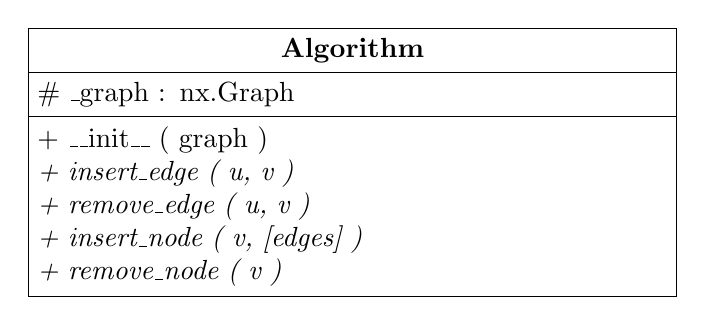
\begin{tikzpicture}
    \begin{class}[text width=8cm]{Algorithm}{0,0}
    \attribute {\# \_graph : nx.Graph}
    \operation {+ \_\_init\_\_ ( graph )}
    \operation [0]{+ insert\_edge ( u, v )}
    \operation [0]{+ remove\_edge ( u, v )}
    \operation [0]{+ insert\_node ( v, [edges] )}
    \operation [0]{+ remove\_node ( v )}
    \end{class}
  \end{tikzpicture}
  \end{center}
\end{frame}

% \section{}
\section{Evaluation}

\begin{frame}{Evaluation: Setup}
  \begin{itemize}
    \item Hardware: Intel Core i7-1065G7
    \item Average time over 5 runs
    \item Time includes initilization and updates
    \item Queries are not performed
      \bigskip
      %\item Comparison with [2] Algorithm was not done
  \end{itemize}
\end{frame}


\begin{frame}{Evaluation: Edge Insertion}
  \begin{table}[]
  \begin{tabular}{|c|c|c|c|c|c|}
    \hline
    Data & Trivial & Simple & Incremental & Dynamic & Implicit \\
    \hline
    \hline
    Wildbirds & 1.281 & 0.013 & 0.012 & 0.064 & 0.020 \\
    \hline
    Topology & DNF & 0.430 & 0.504 & 3.205 & 0.696 \\
    \hline
    Facebook & DNF & 2.582 & 2.228 & DNF & 4.042 \\
    \hline
    Youtube & DNF & 67.058 & 60.695 & DNF & 95.488 \\
    \hline
  \end{tabular}
  \end{table}
  \begin{itemize}
    \item time in seconds
    \item DNF: did not finish after 2 minutes
  \end{itemize}
\end{frame}

\begin{frame}{Evaluation: Insertion Conclusion}
  \begin{itemize}
    \item Function call may have non-negligible overhead
    \item Caching values is important
      \begin{itemize}
        \item edge count
        \item set of heavy nodes
      \end{itemize}
    \item Connect battery to power while benchmarking
  \end{itemize}
\end{frame}

\begin{frame}{Evaluation: Edge Removal}
  \begin{itemize}
    \item Brightkite Friendship Dataset
      \begin{itemize}
        \item 58,228 Nodes
        \item 214,078 Edges
      \end{itemize}
    \item Varying number of edge deletions
    \item Same edges deleted in all runs
  \end{itemize}
\end{frame}

\begin{frame}{Evaluation: Edge Removals}
  \begin{table}[]
  \begin{tabular}{|c|c|c|c|c|c|}
    \hline
    Removals & Trivial & Simple & Dynamic & Implicit \\
    \hline
    \hline
    % 1000 & 2.68 & 0.018 & 0.017 & 0.029 \\
    1000 & 119.539 & 0.219 & 0.253 & 0.280 \\ % the initialisation takes 0.153
    \hline
    10,000 & DNF & 0.259 & 0.441 & 0.433 \\
    \hline
    100,000 & DNF & 0.553 & 2.016 & 1.700 \\
    \hline
  \end{tabular}
  \end{table}
  \begin{itemize}
    \item time in seconds
    \item DNF: did not finish after 2 minutes
    \item Incremental Algorithm does not support edge deletions
  \end{itemize}
\end{frame}


\end{document}
